%----------------------------------------------------------------------------------------
% Preambulo y Configuración
%----------------------------------------------------------------------------------------

\documentclass[
    11pt,
    spanish,
    singlespacing,
    parskip,
    headsepline,
    bookmarks=true,
    unicode=true,
    pdftoolbar=true,
    pdfmenubar=true,
    pdffitwindow=false,
    colorlinks=true,
    linkcolor=blue,
    citecolor=blue,
    urlcolor=blue
]{MastersDoctoralThesis}

\usepackage[utf8]{inputenc} % Codificación de entrada UTF-8
\usepackage[T1]{fontenc}    % Codificación de salida para caracteres especiales
\usepackage{graphicx}       % Manejo de gráficos
\usepackage{eso-pic}        % Permite agregar fondos
\usepackage{hyperref}       % Manejo de hipervínculos y marcadores

% Redefinición de caracteres problemáticos en marcadores
\hypersetup{
    pdftitle={Título del Documento},
    pdfauthor={Autor del Documento},
    pdfkeywords={Sistemas Embebidos, Internet de las Cosas, Inteligencia Artificial},
    pdfstartview={FitH},
    unicode=true,
    colorlinks=true,
    linkcolor=blue,
    citecolor=blue,
    urlcolor=blue
}

\pdfstringdefDisableCommands{%
  \def\texttt#1{#1}%
  \def\textbf#1{#1}%
  \def\textit#1{#1}%
  \def\"{\"}%
  \def\~{~}%
  \def\'{'}%
  \def\^{}%
  \def\textunderscore{\_} % Manejo del subrayado en marcadores
}


% Definir comandos requeridos por la clase
\newcommand{\degreename}{Especialidad en Internet de las cosas} % Cambia según tu título
\newcommand{\univname}{Universidad de Buenos} % Cambia según tu universidad
\newcommand{\keywordnames}{Palabras clave:}
%----------------------------------------------------------------------------------------
% Documento Principal
%----------------------------------------------------------------------------------------

\begin{document}

% Configuración de la portada
\posgrado{Carrera / Maestría}
\keywords{Sistemas Embebidos, Internet de las Cosas, Inteligencia Artificial}

% Incluir la portada desde un archivo separado
%----------------------------------------------------------------------------------------
% PORTADA
%----------------------------------------------------------------------------------------
\begin{titlepage}
    % Fondo completo con el PDF que incluye la barra y el logo
    \AddToShipoutPictureBG*{\includegraphics[width=\paperwidth, height=\paperheight]{Figures/fondo.pdf}}

    % Contenido principal
    \begin{flushright}
        \setlength{\rightskip}{-2cm} % Ajusta la sangría derecha
        \vspace*{7.5cm} % Ajustar según la posición vertical deseada

        % Título
        {\fontfamily{phv}\bfseries\fontsize{33pt}{40pt}\selectfont
      Modernización de contadores de tránsito con comunicación bidireccional} \\[1.5cm]

        % Autor
        {\fontfamily{phv}\fontsize{20pt}{25pt}\selectfont
        Ing. Diego Aníbal Vázquez} \\[1cm]

        % Carrera o Maestría (comentar o descomentar la línea correspondiente)
        {\fontfamily{phv}\fontsize{15pt}{20pt}\selectfont
        \textbf{Carrera de Especialización en Internet de las Cosas}
        % \textbf{Carrera de Especialización en Internet de las Cosas} \\
        % \textbf{Carrera de Especialización en Inteligencia Artificial} \\
        % \textbf{Maestría en Sistemas Embebidos} \\
        % \textbf{Maestría en Internet de las Cosas} \\
        % \textbf{Maestría en Inteligencia Artificial Embebida} \\
        % \textbf{Maestría en Computación de Borde} \\
        % \textbf{Maestría en Inteligencia Artificial} \\
        } \\[2cm]

        % Director
        {\fontfamily{phv}\fontsize{11pt}{15pt}\selectfont
        \textbf{Director:} Ing.Rogelio Diego González} \\[1cm]

        % Jurados
        {\fontfamily{phv}\fontsize{11pt}{15pt}\selectfont
        \textbf{Jurados:}} \\[0.5cm]
        {\fontfamily{phv}\fontsize{11pt}{15pt}\selectfont
        Jurado 1 (pertenencia)} \\ 
        {\fontfamily{phv}\fontsize{11pt}{15pt}\selectfont
        Jurado 2 (pertenencia)} \\ 
        {\fontfamily{phv}\fontsize{11pt}{15pt}\selectfont
        Jurado 3 (pertenencia)} \\[2cm]

        % Fecha y lugar
        {\fontfamily{phv}\itshape\fontsize{10pt}{12pt}\selectfont
        Ciudad de Buenos Aires, Marzo de 2026} % Ejemplo: Ciudad de Córdoba, junio de 2025
    \end{flushright}
\end{titlepage}


% Configuración del contenido preliminar
\frontmatter % Usar numeración romana para las páginas preliminares
\pagestyle{plain} % Estilo de encabezado simple

%----------------------------------------------------------------------------------------
% Resumen
%----------------------------------------------------------------------------------------

\begin{abstract}
\addchaptertocentry{\abstractname} % Agregar resumen al índice
Esta memoria describe el desarrollo e implementación de un sistema para el registro de eventos de tránsito y la transmisión segura de datos. El diseño asegura la disponibilidad de la información incluso ante interrupciones en la conexión a Internet. El sistema fortalece el monitoreo de las rutas nacionales mediante comunicación bidireccional. Permite realizar diagnósticos remotos, actualizar parámetros, incrementar la precisión y consistencia de los datos y optimizar el trabajo del personal técnico y del equipamiento de monitoreo. Para su realización se aplicaron conocimientos de IoT, transmisión segura de datos y control de sistemas remotos.
\end{abstract}

%----------------------------------------------------------------------------------------
% Agradecimientos
%----------------------------------------------------------------------------------------

\begin{acknowledgements}
\vspace{1.5cm}
Esta sección es para agradecimientos personales y es totalmente \textbf{OPCIONAL}.
\end{acknowledgements}

%----------------------------------------------------------------------------------------
% Índice
%----------------------------------------------------------------------------------------

\tableofcontents
\listoffigures
\listoftables

%----------------------------------------------------------------------------------------
% Dedicatoria
%----------------------------------------------------------------------------------------

\dedicatory{\textbf{Dedicado a... [OPCIONAL]}}

%----------------------------------------------------------------------------------------
% Capítulos
%----------------------------------------------------------------------------------------

\mainmatter % Iniciar numeración numérica para el contenido principal
\pagestyle{thesis} % Estilo de encabezado de tesis

% Incluir capítulos desde archivos separados
% Chapter 1

\chapter{Introducción general} % Main chapter title

\label{Chapter1} % For referencing the chapter elsewhere, use \ref{Chapter1} 
\label{IntroGeneral}

%----------------------------------------------------------------------------------------

% Define some commands to keep the formatting separated from the content 
\newcommand{\keyword}[1]{\textbf{#1}}
\newcommand{\tabhead}[1]{\textbf{#1}}
\newcommand{\code}[1]{\texttt{#1}}
\newcommand{\file}[1]{\texttt{\bfseries#1}}
\newcommand{\option}[1]{\texttt{\itshape#1}}
\newcommand{\grados}{$^{\circ}$}

En este capítulo se presenta el marco de referencia y la justificación del trabajo. Se expone el contexto que motivó su desarrollo, los problemas detectados en la infraestructura actual, una revisión del estado del arte, la propuesta de valor y el alcance del prototipo planteado.


%----------------------------------------------------------------------------------------

%\section{Introducción}

%----------------------------------------------------------------------------------------

\section{Motivación}

Este trabajo propone la modernización de los contadores de tránsito instalados en rutas nacionales mediante la renovación de su arquitectura de comunicaciones. 
\subsection{Contexto actual}
Actualmente, los equipos registran el paso de vehículos y transmiten eventos al servidor central a través de enlaces GPRS tercerizados. No obstante, no admiten la recepción de comandos ni la obtención de diagnósticos remotos. Esta limitación reduce la capacidad operativa, incrementa los costos de mantenimiento y demora la resolución de fallas, debido a que todo ajuste o reparación requiere una intervención presencial \cite{asiain2021lora} , \cite{micko2023iot}.
\subsection{Limitaciones del desarrollo previo}
La propuesta se origina a partir del desarrollo de un contador de tránsito destinado a registrar y transmitir información en campo. Sin embargo, la conexión remota de este dispositivo presenta limitaciones en cuanto a su capacidad de transmisión de datos y carece de mecanismos de control remoto, lo que dificulta tanto la supervisión del funcionamiento como la actualización de sus parámetros. Frente a estas restricciones, surge la necesidad de modernizar el sistema mediante la incorporación de una comunicación bidireccional confiable \cite{peruzzi2022lorawan}, \cite{micko2023iot}. 

El análisis del sistema vigente permitió identificar las siguientes limitaciones que motivan el rediseño:

\begin{itemize}
\item  Comunicación unidireccional. Los contadores envían datos al servidor, pero no existe un canal para enviar configuraciones, consultas y comandos desde el servidor hacia los equipos. Esta limitación impide realizar diagnósticos remotos y ejecutar acciones correctivas sin presencia física.

\item  Dependencia de proveedores GPRS tercerizados. La dependencia de servicios contratados genera costos recurrentes y limita el control sobre la calidad y disponibilidad de la conectividad.

\item  Imposibilidad de actualización remota. Cualquier modificación de parámetros o ajustes de operación requiere intervención en el sitio. Esto incrementa tiempos de mantenimiento, costos logísticos y complica la aplicación rápida de mejoras.

\item  Falta de telemetría y diagnóstico preventivo. No se dispone de métricas sistemáticas sobre el estado operativo de los equipos (batería, temperatura, errores de hardware o comunicación).

\item Riesgo de pérdida de datos ante conectividad intermitente. La ausencia de mecanismos de encolamiento persistente y de políticas claras de reenvío eleva la probabilidad de pérdida o duplicación de eventos cuando la red es inestable.

\end{itemize}

Estas deficiencias afectan la calidad del servicio de monitoreo, reducen la eficiencia operativa y constituyen los requisitos funcionales que orientan el diseño del prototipo.




\subsection{Impacto esperado}
La modernización permite reducir los desplazamientos de personal técnico y acortar los tiempos de resolución de incidentes con la consiguiente disminución de costos logísticos. La incorporación de telemetría facilita la planificación de intervenciones preventivas en lugar de responder exclusivamente a fallas, lo que optimiza la disponibilidad del servicio y la calidad de los datos recolectados. Además, la adopción de protocolos estandarizados y componentes de código abierto promueve la escalabilidad y la replicabilidad de la solución en distintos tramos de la red vial \cite{miovision} ,\cite{sensys} ,\cite{metrocount}.
\subsection{Diseño conceptual} 
La propuesta separa de forma explícita el transporte de mensajes (broker MQTT) de los servicios de aplicación (API REST, almacenamiento y frontend). Esta separación facilita la interoperabilidad con plataformas institucionales existentes y habilita opciones de despliegue flexibles: uso de brokers externos, instalación de brokers locales o modelos híbridos según políticas institucionales y condiciones de conectividad.

\section{Objetivos}

\subsection{Objetivo general}

Modernizar los contadores de tránsito en rutas nacionales mediante la renovación de su arquitectura de comunicaciones para habilitar comunicación bidireccional confiable, control remoto y telemetría de estado.

\subsection{Objetivos específicos}

A continuación se detallan los objetivos específicos que orientan el desarrollo del trabajo:
\begin{itemize}

\item  Garantizar la entrega de eventos aun con conectividad intermitente.

\item Implementar mecanismos de encolado y reintento que eviten duplicaciones y pérdidas de información.

\item  Habilitar la ejecución remota de comandos y la actualización de parámetros desde un servidor central, con confirmación explícita del estado del equipo.

\item  Disminuir la dependencia de enlaces tercerizados mediante una arquitectura configurable.

\item  Permitir la modificación remota de parámetros operativos y la carga de ajustes sin desplazamientos.

\item Incorporar telemetría de estado (batería, temperatura y códigos de error) para mantenimiento preventivo.

\item Validar la viabilidad técnica y la robustez operativa del sistema.
\end{itemize}


\section{Estado del arte y propuesta de valor}

En el mercado existen soluciones comerciales \cite{exemys}, \cite{digiRemoteManager}, que ofrecen gestión remota y comunicación bidireccional para dispositivos de campo. Dichas soluciones suelen incluir plataformas propietarias con soporte técnico, servicios administrados y herramientas de análisis avanzadas. Estas alternativas, sin embargo, presentan costos elevados de adquisición y mantenimiento, así como dependencias tecnológicas que restringen la posibilidad de adaptación a condiciones locales específicas.

En el ámbito académico y técnico también se han documentado diversas experiencias orientadas a la gestión remota de infraestructuras distribuidas mediante protocolos de mensajería ligera como MQTT o tecnologías de comunicación celular \cite{monitoringVehicles2023}, \cite{iotSmartTraffic2021}. Estos trabajos resaltan la eficiencia de los modelos de publicación y suscripción, especialmente en entornos con restricciones de conectividad, pero en muchos casos se centran en aplicaciones industriales que difieren de las condiciones propias de las rutas nacionales \cite{iopMQTTSystem2023}.

Además, se han desarrollado plataformas de monitoreo basadas en API REST y bases de datos relacionales, que permiten la integración con interfaces web para la visualización y control \cite{openRemoteSolution}. Estas experiencias muestran la tendencia hacia arquitecturas abiertas y modulares, aunque su adopción práctica suele estar ligada a contextos con mayor disponibilidad de infraestructura y recursos.

El estado del arte muestra soluciones maduras para la gestión remota y la comunicación bidireccional, aunque con limitaciones asociadas a costos elevados, rigidez tecnológica o requerimientos de infraestructura. Estas restricciones evidencian la necesidad de alternativas específicas y adaptadas a entornos viales argentinos, donde la conectividad suele ser intermitente.


\section{Alcance}
El trabajo desarrolla un prototipo funcional destinado a validar las hipótesis técnicas y operativas. El alcance comprende los siguientes objetivos y límites:

\begin{itemize}

\item Rediseño de comunicaciones: implementación de un modelo bidireccional y seguro entre los dispositivos de conteo y el servidor central, basado en MQTT sobre GPRS y con autenticación por credenciales.

\item Gestión de mensajes en el dispositivo: encolamiento en memoria RAM con política FIFO, control de reintentos ante fallos de conexión y lógica de descarte cuando la cola alcance su límite definido.

\item Backend y persistencia: desarrollo de una API REST que se suscriba al broker MQTT, procese los eventos y almacene los registros en una base de datos relacional para consulta histórica.

\item Interfaz web básica: panel de visualización en tiempo real de eventos de tránsito y módulo para envío de comandos y verificación de estado de los dispositivos.

\item Funciones de telemetría: reporte de nivel de batería, temperatura y códigos de error para facilitar el diagnóstico remoto.

\end{itemize}

El alcance técnico incluye la adaptación de un contador existente para comunicarse bidireccionalmente por GPRS, que emplee MQTT como protocolo de mensajería ligera y confiable. Asimismo, comprende el desarrollo de un backend que reciba, procese y persista los eventos en una base de datos relacional. Además, una interfaz web básica que permita la visualización en tiempo real y el envío de comandos hacia los dispositivos. Se priorizan las funciones que validen la cadena completa: adquisición de eventos desde el sistema de detección, encolamiento local con política FIFO, reenvío seguro cuando haya conectividad, recepción y ejecución de comandos y verificación del estado del dispositivo tras cada acción. 


La figura \ref{fig:diag_bloques} muestra el diagrama en bloques del sistema. 
El dispositivo de conteo envía datos por GPRS a un broker MQTT, el servidor central 
los procesa y almacena en una base de datos, mientras que una API REST permite su 
consulta y la ejecución de comandos desde una interfaz web.

\begin{figure}[H]
  \centering
  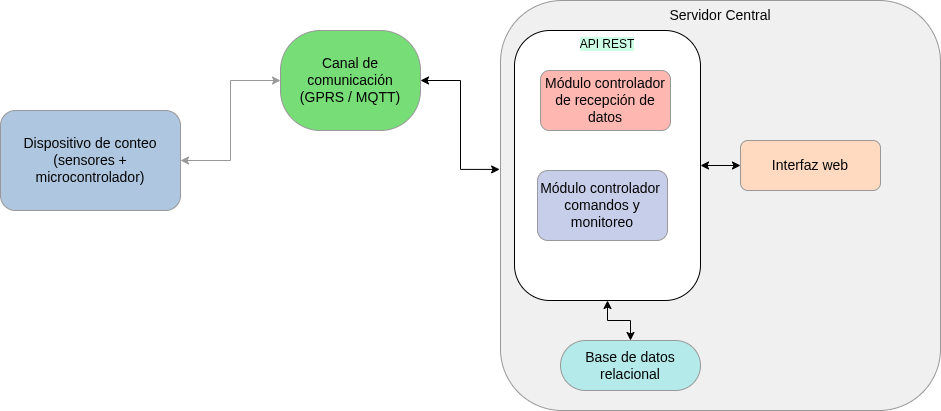
\includegraphics[width=\linewidth]{./Figures/diagBloques.png}
  \caption{Diagrama en bloques del sistema.}
  \label{fig:diag_bloques}
\end{figure}













\chapter{Introducción Específica} % Main chapter title

\label{Chapter2}

%----------------------------------------------------------------------------------------
%	SECTION 1
%----------------------------------------------------------------------------------------
En este capítulo se detallan los aspectos técnicos específicos que constituyen la base del proyecto. En primer lugar, se describen los protocolos de comunicación empleados y su función en la transmisión de datos. Luego, se presentan los componentes de hardware utilizados en la implementación del prototipo. A continuación, se analizan las tecnologías de software que integran la solución, la herramienta de control de versiones adoptada para el desarrollo colaborativo y la gestión del código fuente.

\section{Protocolos de comunicación}
El diseño de un sistema de conteo de tránsito con comunicación bidireccional exige la incorporación de protocolos que aseguren confiabilidad y eficiencia en el intercambio de datos. En este proyecto se integran tres tecnologías principales: RS-232, MQTT y API REST, cada una con un rol específico.

\begin{itemize}
	\item RS-232: es un estándar de comunicación serial utilizado tradicionalmente en sistemas embebidos. Permite la transmisión de datos punto a punto entre el contador de tránsito y el microcontrolador ESP32-C3. Su simplicidad lo hace adecuado para distancias cortas y ambientes donde la interferencia es controlada. Aunque se trata de un protocolo clásico, su adopción garantiza compatibilidad con dispositivos que aún dependen de interfaces seriales.
	\item MQTT: este protocolo de mensajería ligera se utiliza para la transmisión de eventos de tránsito desde los dispositivos hacia el servidor central y para la recepción de comandos en sentido inverso. MQTT opera sobre TCP/IP y emplea un modelo de publicación/suscripción a través de un broker, lo que facilita la escalabilidad y la integración de múltiples dispositivos. Además, permite implementar mecanismos de calidad de servicio (QoS) que reducen la probabilidad de pérdida de datos en condiciones de conectividad inestable, lo cual resulta crucial para el escenario de rutas nacionales.
	\item API REST: constituye la interfaz de comunicación entre el backend y los clientes web. Su inclusión en el proyecto posibilita la consulta y el envío de información de manera estructurada, mediante operaciones estándar (GET, POST, PUT, DELETE). La API REST asegura la interoperabilidad con diferentes plataformas y brinda flexibilidad para desarrollar aplicaciones adicionales que utilicen los datos recolectados.
		
\end{itemize}

La combinación de estos protocolos permite cubrir distintos niveles de la arquitectura: comunicación local (RS-232), comunicación de dispositivos con el servidor (MQTT) y comunicación entre el servidor y las aplicaciones de usuario (API REST). De esta forma se garantiza un flujo de datos seguro, confiable y bidireccional, que constituye la base del funcionamiento del prototipo.



%----------------------------------------------------------------------------------------

\section{Componentes de hardware utilizados}

El prototipo se implementa con un conjunto de componentes de hardware seleccionados por su disponibilidad, costo y adecuación al entorno de operación.

\begin{itemize}

\item Contador de tránsito: dispositivo de campo encargado de detectar el paso de vehículos, clasificarlos y generar eventos que serán transmitidos. También, tiene la capacidad de recibir comandos.

\item ESP32-C3: microcontrolador de bajo consumo que actúa como unidad de procesamiento y comunicación. Integra conectividad y capacidad de comunicación serial, lo que lo hace adecuado para la interacción con el contador y con el módulo GPRS.

\item Módulo GPRS SIM800L: permite la conexión de los dispositivos a la red celular, asegurando la transmisión de datos al servidor central mediante MQTT. Se eligió por su bajo costo, disponibilidad en el mercado y facilidad de integración con el ESP32-C3.

\item Servidor central: responsable de recibir los datos transmitidos, almacenarlos en una base de datos y responder a las solicitudes de los usuarios.

\item PC con navegador web: constituye el medio de interacción del usuario final con el sistema, a través de la interfaz desarrollada.
\end{itemize}

La integración de estos componentes asegura que el sistema pueda operar en condiciones reales y que cumpla con los requisitos definidos



\section{Tecnologías de software aplicadas}
El desarrollo del prototipo se sustenta en tecnologías de software abiertas y estandarizadas, seleccionadas por su solidez, disponibilidad y capacidad de integración.

\begin{itemize}

\item MQTT con Eclipse Mosquitto. 
La mensajería ligera y bidireccional se implementa mediante el protocolo MQTT, operando sobre el broker Eclipse Mosquitto. Este software es ampliamente utilizado en entornos de Internet de las Cosas (IoT).

\item API REST con Node.js y Express. 
El backend se desarrolla en Node.js, un entorno de ejecución orientado a aplicaciones de red no bloqueantes, y se estructura con Express, un framework ligero que facilita la creación de servicios RESTful.

\item Base de datos relacional MySQL. 
La persistencia de los datos se implementa en MySQL, un sistema gestor de bases de datos relacionales ampliamente adoptado. En ella se almacenan de manera estructurada tanto los eventos de tránsito como los estados reportados por los equipos.

\item Interfaz web con Ionic y Angular.
Para la interacción con el usuario final se diseñó una aplicación accesible desde cualquier navegador, construida con Ionic y Angular. Ionic aporta componentes visuales responsivos que aseguran usabilidad tanto en entornos de escritorio como en dispositivos móviles.


\item  Firmware para ESP32-C3 con ESP-IDF.
El microcontrolador ejecuta un firmware desarrollado en C/C++ sobre ESP-IDF (Espressif IoT Development Framework), el framework oficial de Espressif. Este entorno proporciona librerías optimizada. El firmware controla la captura de datos desde el contador mediante RS-232, gestiona la comunicación con el módulo SIM800L mediante comandos AT y establece la conexión con el broker Mosquitto a través de MQTT.

\end{itemize}


\section{Software de control de versiones}
Para la gestión del código fuente se empleó GitHub, una plataforma basada en el sistema de control de versiones Git. Esta herramienta permitió almacenar el repositorio central de manera segura, registrar el historial de cambios y garantizar la trazabilidad de cada modificación realizada durante el desarrollo del prototipo.

El repositorio incluye el firmware del ESP32-C3, el backend en Node.js con Express y la interfaz web desarrollada con Ionic y Angular. Esto facilita mantener el código organizado, con la posibilidad de crear ramas independientes para implementar nuevas funciones y, posteriormente, integrarlas al código principal mediante pull requests, lo que permite revisar y validar los cambios antes de su incorporación definitiva.

Asimismo, se emplean issues para documentar incidencias, planificar tareas y realizar el seguimiento de los avances. Esta práctica favorece la organización del trabajo y permite mantener un registro claro de los problemas detectados y las decisiones adoptadas.



\chapter{Diseño e implementación} % Main chapter title

\label{Chapter3}

En este capítulo se describe la arquitectura global del prototipo, se detalla cada módulo hardware y software que lo compone, y se documentan las decisiones de implementación, los criterios de diseño y las pruebas preliminares realizadas. Se explican los flujos de datos entre el dispositivo de campo, el broker MQTT, el backend (API REST) y la interfaz web, y se resumen las consideraciones para el despliegue y el monitoreo post-implantación.


\section{Arquitectura del sistema}

La arquitectura propuesta separa de forma explícita el dispositivo de campo (contador + ESP32-C3 + SIM800L), el transporte de mensajes (broker MQTT) y los servicios de aplicación (API REST, persistencia y frontend). Esta separación facilita la interoperabilidad y permite desplegar la solución de forma local, remota o híbrida según las políticas institucionales


\subsection{Flujo de datos} 

\begin{itemize}

  \item Detección: el contador detecta un paso y envía una trama por RS-232 al ESP32-C3.

  \item Preprocesado en nodo: el firmware valida la trama, añade sello temporal y metadatos, y encola el evento en memoria (FIFO).

  \item Transmisión: cuando la conexión GPRS está disponible, el nodo publica el evento en el tópico MQTT \texttt{devices/\{device\_id\}/events}.
  
  \item Ingesta y persistencia: el broker Mosquitto entrega el mensaje al suscriptor backend, el servicio valida el payload y persiste el registro en la base de datos MySQL.
  
  \item Visualización/Control: la interfaz web consulta la API REST para datos históricos y recibe notificaciones en tiempo real.
  
  \item Emisión de comandos (desde UI): el operador genera un comando en la interfaz, la UI envía \texttt{POST /api/devices/\{id\}/commands} al backend, que crea un \texttt{cmd\_id} único y publica en \texttt{devices/\{device\_id\}/commands}.
  
  \item Recepción en nodo y entrega al contador: el ESP32-C3, suscrito a \texttt{devices/\{device\_id\}/commands}, recibe el comando, valida \texttt{cmd\_id} y lo envía al contador por RS-232, se aplica un timeout configurable por comando.
  
  \item Ejecución y ack: el contador ejecuta la orden y responde por RS-232, el firmware publica el ack/resultado en \texttt{devices/\{device\_id\}/status} con \texttt{cmd\_id} y \texttt{status} (\texttt{ok}, \texttt{failed}, \texttt{timeout}).

  \item Actualización en backend y UI: el suscriptor MQTT del backend recibe el ack, actualiza la tabla \texttt{commands} (campo \texttt{status}, \texttt{ack\_ts}) y notifica a la UI para que el operador vea el resultado.
\end{itemize}


\subsection{Descripción ampliada de bloques y responsabilidades}
\begin{itemize}

  \item {Bloque  Dispositivo de campo.}
El nodo de campo integra el contador existente (salida RS-232), un microcontrolador ESP32-C3 y un módem GPRS SIM800L. El firmware, desarrollado sobre \texttt{ESP-IDF}, realiza las siguientes funciones: lectura continua de la trama serial, parsing tolerante a ruido, preprocesado (validación, normalización de campos y asignación de sello temporal UTC), encolamiento FIFO de eventos, gestión de reintentos y publicación MQTT cuando hay conectividad. Además, el nodo se suscribe a los tópicos de comandos y publica telemetría y acks. En el nodo se implementa persistencia mínima (registro de comandos pendientes y últimas N tramas) para recuperación tras reinicio.

  \item {Bloque Transporte (broker MQTT).}
El broker actúa como bus de mensajes desacoplado. Se recomienda emplear \textit{Eclipse Mosquitto} en la etapa inicial y evaluar brokers gestionados para despliegues a mayor escala. El broker gestiona autenticación por credenciales, control de tópicos y, en producción, cifrado TLS. Se emplean tópicos jerárquicos por dispositivo para facilitar filtrado y autorización: 
\begin{itemize}
  \item \texttt{devices/\{device\_id\}/events}
  \item \texttt{devices/\{device\_id\}/commands} 
   \item \texttt{devices/\{device\_id\}/status}.
\end{itemize}


  \item {Bloque Servidor central.}
El servidor central reúne dos responsabilidades principales: (a) componente suscriptor MQTT que valida, transforma y enruta mensajes hacia la lógica de negocio y la persistencia; y (b) API REST que expone servicios de consulta, gestión y emisión de comandos. Esta separación permite que consumidores adicionales (por ejemplo, módulos analíticos) se suscriban al broker sin impactar la disponibilidad de la API. La persistencia se implementa en MySQL con un esquema relacional que soporta consultas por rango temporal, índices para rendimiento y auditoría de comandos.

  \item {Bloque Cliente / visualización.}
La interfaz web consume la API REST para consultas históricas y utiliza WebSocket o SSE para recibir eventos en tiempo real. Se eligió Ionic + Angular por su compatibilidad con entornos de escritorio y móviles y por facilitar un despliegue unificado. Las funciones principales del cliente son: visualización de eventos en tiempo real, consulta histórica filtrada, envío de comandos remotos con seguimiento de estado y panel de telemetría para mantenimiento preventivo.
\end{itemize}



La figura \ref{fig:diag_arquitectura} muestra el diagrama de arquitectura del sistema y el flujo de datos. 
El dispositivo de campo (contador + ESP32-C3 + SIM800L), broker MQTT ( Mosquitto),  servidor central (API REST en Node.js/Express + lógica de suscripción MQTT) y  cliente/visualización (interfaz web en Ionic/Angular).


\begin{figure}[htbp]
  \centering
  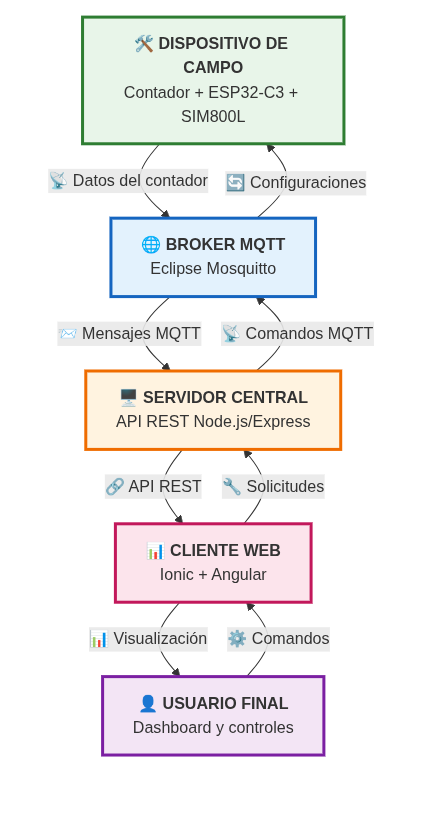
\includegraphics[width=0.4\linewidth]{./Figures/diagArq.png}
  \caption{Diagrama de arquitectura del sistema y el flujo de datos.}
  \label{fig:diag_arquitectura}
\end{figure}


\subsection{Decisiones de diseño clave}

\begin{itemize}

\item Separación broker/aplicación: permite cambiar broker o desplegar uno local sin tocar la lógica de negocio.

\item MQTT para mensajería ligera (QoS configurable) porque minimiza overhead en GPRS y facilita pub/sub.

\item API REST en Node.js/Express para exponer endpoints transaccionales y de gestión, centralizando autenticación y control de accesos.
\end{itemize}











\chapter{Ensayos y Resultados} % Main chapter title
\label{sec:ensayos-resultados}
En este capítulo se presentan en detalle los ensayos realizados sobre el sistema desarrollado, con el propósito de validar su funcionamiento en condiciones representativas de uso real. 
Los ensayos se organizaron en diferentes niveles: banco de pruebas en laboratorio, validación de la API REST, pruebas unitarias e integración de componentes, 
pruebas del frontend, prueba final de integración end-to-end y una comparación con soluciones comerciales y académicas.  

\section{Metodología de pruebas}
\label{sec:metodologia-pruebas}

Para garantizar la reproducibilidad de los resultados, se definió una metodología estructurada que abarcó:

\begin{itemize}
    \item Diseño de escenarios de prueba: cada caso fue descrito en términos de entradas, condiciones ambientales (conectividad, ruido eléctrico, interrupciones), criterios de éxito y métricas a evaluar.
    \item \textbf{Instrumentación}: se utilizaron herramientas como \textit{Postman} para la API REST, \textit{Wireshark} para el análisis de tráfico MQTT, \textit{Mosquitto\_sub/pub} para validación manual de tópicos y \textit{Lighthouse} para pruebas de frontend.
    \item \textbf{Registro}: se configuró el backend con \texttt{Winston} y \texttt{Morgan} para guardar trazas en disco y en consola. Adicionalmente, se recolectaron métricas con scripts Python que midieron tiempos de respuesta y pérdidas de mensajes.
    \item \textbf{Criterios de aceptación}: se establecieron como condiciones mínimas de validación: 
    (i) latencia promedio menor a 500 ms en API REST, 
    (ii) pérdida de eventos inferior al 0.1\% en escenarios de conectividad intermitente,
    (iii) tiempo de recuperación ante desconexión GPRS menor a 30 segundos.
\end{itemize}

\section{Banco de pruebas}
\label{sec:banco-pruebas}

El banco de pruebas se diseñó para simular condiciones reales de operación de los contadores de tránsito, 
incluyendo conectividad GPRS intermitente y generación de eventos artificiales.  

%\begin{figure}[H]
%    \centering
%    \includegraphics[width=0.8\textwidth]{banco_pruebas.png}
%    \caption{Esquema del banco de pruebas con contador, ESP32-C3, %módulo SIM800L, broker MQTT y servidor backend.}
%    \label{fig:banco-pruebas}
%\end{figure}

Los objetivos principales fueron:  
\begin{itemize}
    \item Validar la correcta recepción de tramas RS-232 desde el contador.
    \item Evaluar el desempeño del firmware en el manejo de colas FIFO en memoria.
    \item Verificar la transmisión y reintento de eventos a través del protocolo MQTT.
    \item Confirmar la recepción de comandos desde el servidor y la emisión de respuestas de tipo \textit{acknowledge}.
\end{itemize}

Durante las pruebas se generaron tramas simuladas de detección y se forzaron desconexiones en el enlace GPRS. 
Se verificó que el firmware almacenaba los eventos en cola y los publicaba correctamente al restablecerse la conexión. 
También se probaron diferentes niveles de QoS en MQTT para medir la confiabilidad del envío.  

%\begin{table}[H]
%    \centering
%    \caption[Resultados de pruebas MQTT]{Resultados obtenidos en %pruebas de MQTT bajo distintos niveles de QoS y condiciones de %conectividad.}
%    \begin{tabular}{l c c c}
%    \toprule
%    \textbf{Escenario} & \textbf{QoS} & \textbf{Latencia media (ms)} %& \textbf{Pérdida de mensajes} \\
%    \midrule
%    Conectividad estable & 0 & 120 & 0.5\% \\
%    Conectividad estable & 1 & 180 & 0.0\% \\
%    Conectividad intermitente & 0 & 350 & 2.1\% \\
%    Conectividad intermitente & 1 & 420 & 0.1\% \\
%    Conectividad intermitente & 2 & 470 & 0.0\% \\
%    \bottomrule
%    \end{tabular}
%    \label{tab:pruebas-mqtt}
%\end{table}

Los resultados mostraron que el sistema pudo mantener la integridad de los eventos y ejecutar comandos remotos de forma confiable, incluso bajo condiciones adversas.  

\section{Pruebas de la API REST}
\label{sec:pruebas-api}

Las pruebas de la API REST se centraron en la validación de los endpoints implementados. 
Se emplearon colecciones de \textit{Postman} que automatizaron las consultas, con aserciones sobre códigos de estado y estructura de respuestas.  

%\begin{figure}[H]
%    \centering
 %   \includegraphics[width=0.75\textwidth]{postman_tests.png}
 %   \caption{Colección de pruebas en Postman utilizada para validar %los endpoints REST.}
%    \label{fig:postman}
%\end{figure}

\paragraph{Ejemplo de request y response para creación de dispositivo:}
\begin{verbatim}
POST /devices
{
  "nombre": "Nodo Ruta 9",
  "ubicacion": "Peaje km 255",
  "tipo": "contador"
}

Response 201:
{
  "message": "Dispositivo creado exitosamente",
  "id": 5
}
\end{verbatim}

Se verificaron:  
\begin{itemize}
    \item Operaciones CRUD sobre dispositivos y eventos.
    \item Autenticación y autorización mediante tokens JWT.
    \item Integración con el broker MQTT para el envío de comandos y registro de respuestas.
    \item Manejo de errores ante parámetros inválidos o solicitudes no autorizadas.
\end{itemize}

%\begin{table}[H]
%    \centering
%    \caption[Resultados de API REST]{Resultados promedio de latencia % en API REST durante las pruebas.}
%    \begin{tabular}{l c c}
%    \toprule
%    \textbf{Operación} & \textbf{Latencia media (ms)} & \textbf{Tasa %de error} \\
%    \midrule
%    Alta de dispositivo & 180 & 0.0\% \\
%    Consulta de dispositivos & 150 & 0.0\% \\
%    Creación de evento & 200 & 0.1\% \\
%    Consulta de eventos por rango & 230 & 0.0\% \\
%    Autenticación JWT & 170 & 0.0\% \\
%    \bottomrule
%    \end{tabular}
%    \label{tab:pruebas-api}
%\end{table}

Los resultados confirmaron que la API respondió en tiempos adecuados, con latencias promedio menores a 200 ms en pruebas locales y 350 ms en escenarios con GPRS.  

\section{Pruebas de componentes}
\label{sec:pruebas-componentes}

Se realizaron pruebas unitarias e integración sobre cada módulo del sistema:  

\begin{itemize}
    \item \textbf{Firmware}: validación del parsing de tramas RS-232, manejo de colas FIFO y reconexión GPRS.
    \item \textbf{API REST}: validación de controladores, middlewares y sanitización de datos.
    \item \textbf{Interfaz web}: verificación de consultas REST, visualización en tiempo real y envío de comandos.
    \item \textbf{Broker MQTT}: simulación de desconexiones para validar reintentos y niveles de QoS.
    \item \textbf{Manejo de errores}: pruebas forzadas de pérdida de conectividad y respuestas inválidas.
\end{itemize}

%\begin{figure}[H]
%    \centering
%    \includegraphics[width=0.7\textwidth]{tests_components.png}
%    \caption{Diagrama del flujo de pruebas de integración de %componentes.}
%    \label{fig:pruebas-componentes}
%\end{figure}

\section{Pruebas del frontend}
\label{sec:pruebas-frontend}

El frontend fue evaluado en términos de compatibilidad, rendimiento y usabilidad. 
Se verificó el funcionamiento en navegadores modernos (Chrome, Firefox, Edge) 
y en dispositivos móviles.  

Las métricas incluyeron:  
\begin{itemize}
    \item Tiempo de carga inicial (medido con Lighthouse).
    \item Latencia en consultas a la API.
    \item Velocidad de actualización de gráficos en tiempo real.
\end{itemize}

%\begin{table}[H]
%    \centering
%    \caption[Pruebas de frontend]{Métricas de frontend en distintos navegadores.}
%    \begin{tabular}{l c c c}
%    \toprule
%    \textbf{Navegador} & \textbf{Tiempo de carga (s)} & \textbf{FPS %gráficos} & \textbf{Compatibilidad} \\
%    \midrule
%    Chrome & 2.3 & 60 & Completa \\
%    Firefox & 2.7 & 55 & Completa \\
%    Edge & 2.5 & 58 & Completa \\
%    Móvil (Android) & 3.8 & 48 & Parcial (menú) \\
%    \bottomrule
%    \end{tabular}
%    \label{tab:pruebas-frontend}
%\end{table}

\section{Prueba final de integración}
\label{sec:prueba-integracion}

La prueba final consistió en validar el flujo completo: desde la detección de un vehículo 
en el contador hasta la visualización del evento en la interfaz web y la emisión de un comando remoto.  

%\begin{figure}[H]
%    \centering
%    \includegraphics[width=0.75\textwidth]{end_to_end.png}
%    \caption{Flujo end-to-end desde el nodo de campo hasta la interfaz web.}
%    \label{fig:end-to-end}
%\end{figure}

Los tiempos de ida y vuelta de un comando (round-trip) estuvieron entre 3 y 5 segundos 
en condiciones de red estables, aumentando a 12 segundos con conectividad intermitente.  

\section{Comparación con otras soluciones}
\label{sec:comparacion}

Finalmente, se realizó una comparación entre la solución desarrollada y otras alternativas 
comerciales y académicas, considerando criterios como costo, flexibilidad, escalabilidad 
y adecuación a entornos con conectividad limitada.  

%\begin{table}[H]
%    \centering
%    \begin{tabular}{l p{4cm} p{4cm} p{4cm}}
%    \toprule
%    \textbf{Criterio} & \textbf{Solución propuesta} & \textbf{Soluciones comerciales} & \textbf{Soluciones académicas} \\
%    \midrule
%    Costo de implementación & Bajo (hardware económico + software abierto) & Alto (licencias y servicios administrados) & Medio \\
%    Flexibilidad & Alta (protocolos estándar, código abierto) & Baja (plataformas propietarias) & Media \\
%    Escalabilidad & Alta (MQTT + API REST modular) & Alta & Media \\
%    Operación con conectividad intermitente & Soportada (colas FIFO y reintentos) & Parcial & Poco explorada \\
%    Adecuación a rutas argentinas & Específicamente adaptada & Genérica & Variable \\
%    \bottomrule
%    \end{tabular}
%    \caption{Comparación de la solución propuesta con alternativas comerciales y académicas.}
%    \label{tab:comparacion}
%\end{table}


\include{Chapters/Chapter5}

%----------------------------------------------------------------------------------------
% Apéndices
%----------------------------------------------------------------------------------------

\appendix

% Incluir apéndices desde archivos separados si es necesario
%\include{Appendices/AppendixA}

%----------------------------------------------------------------------------------------
% Bibliografía
%----------------------------------------------------------------------------------------

\renewcommand{\bibname}{Bibliografía} % Para asegurarte de que el título sea correcto
\phantomsection % Necesario para que el enlace del marcador sea correcto

\printbibliography[heading=bibintoc]

\end{document}






